\documentclass[main.tex]{subfiles}
\begin{document}

\section{Verified Figure Section}
\label{sec:verified-figure-section}

This section inserts only figure files that were verified on disk and that can be tied back to the aligned dataset, the diagnostics tables, or the generating scripts. The repository contains 792 raw specimen images under \path{Data/Images_dataset/} and 94 generated PNG report figures under \path{outputs/}. The curated set below uses 15 image files: 2 raw source images and 13 generated figures. No microscopy micrographs, specimen-preparation photographs, or direct mechanical-test photographs were found, so those figure types are recorded explicitly as absent rather than reconstructed.

\subsection{Experimental setup and specimen overview}

The repository does not contain a dedicated laboratory setup photograph, camera-rig figure, or saved segmentation-overlay figure. The most defensible entry point is therefore the raw longitudinal image corpus itself. Figure~\ref{figsec:raw-d01} shows two aligned source images for specimen \texttt{D01} from \texttt{campaign\_2}; both files are linked in \path{outputs/data/master_table.csv} to week 0 and week 36 observations. The elongated image geometry is also the basis of the strip-wise feature extraction in \path{src/corrosion_proxy_rul/image_features.py}, where image width is mapped to the nominal 24~cm specimen length configured in \path{configs/features.yaml}.

\begin{figure}[t]
    \centering
    
\includegraphics[width=0.49\textwidth]{Data/Images_dataset/D01-20240110-0W.png}\hfill
    
\includegraphics[width=0.49\textwidth]{Data/Images_dataset/D01-20240918-36W.png}
    \caption{Raw longitudinal source images for specimen \texttt{D01} at week 0 (left; \texttt{D01-20240110-0W.png}) and week 36 (right; \texttt{D01-20240918-36W.png}). These are aligned observation images rather than generated diagnostics. The later image shows more rust-coloured staining and localized patches, which is consistent with the increase in stored \texttt{peak\_rust\_pct} for this specimen from 0.020 at week 0 to 2.940 at week 36 in the aligned table. The figure does not reveal subsurface steel loss or residual load capacity.}
    \label{figsec:raw-d01}
\end{figure}

What can be concluded from Figure~\ref{figsec:raw-d01} is limited to visible surface condition and the image format that the pipeline actually receives. A single specimen pair cannot stand in for the full cohort. The broader repository includes low-change specimens such as \texttt{G04} and sharply accelerating specimens such as \texttt{S2SA03} and \texttt{D04}, so the temporal figures below are required before making any statement about corrosion progression at campaign level.

\subsection{Dataset constraints and verified supervision}

The first figure family explains why the project is staged into visible-corrosion, hidden-damage, degradation, and proxy-RUL layers. Figure~\ref{figsec:data-availability} combines the repository's two clearest availability plots.

\begin{figure}[t]
    \centering
    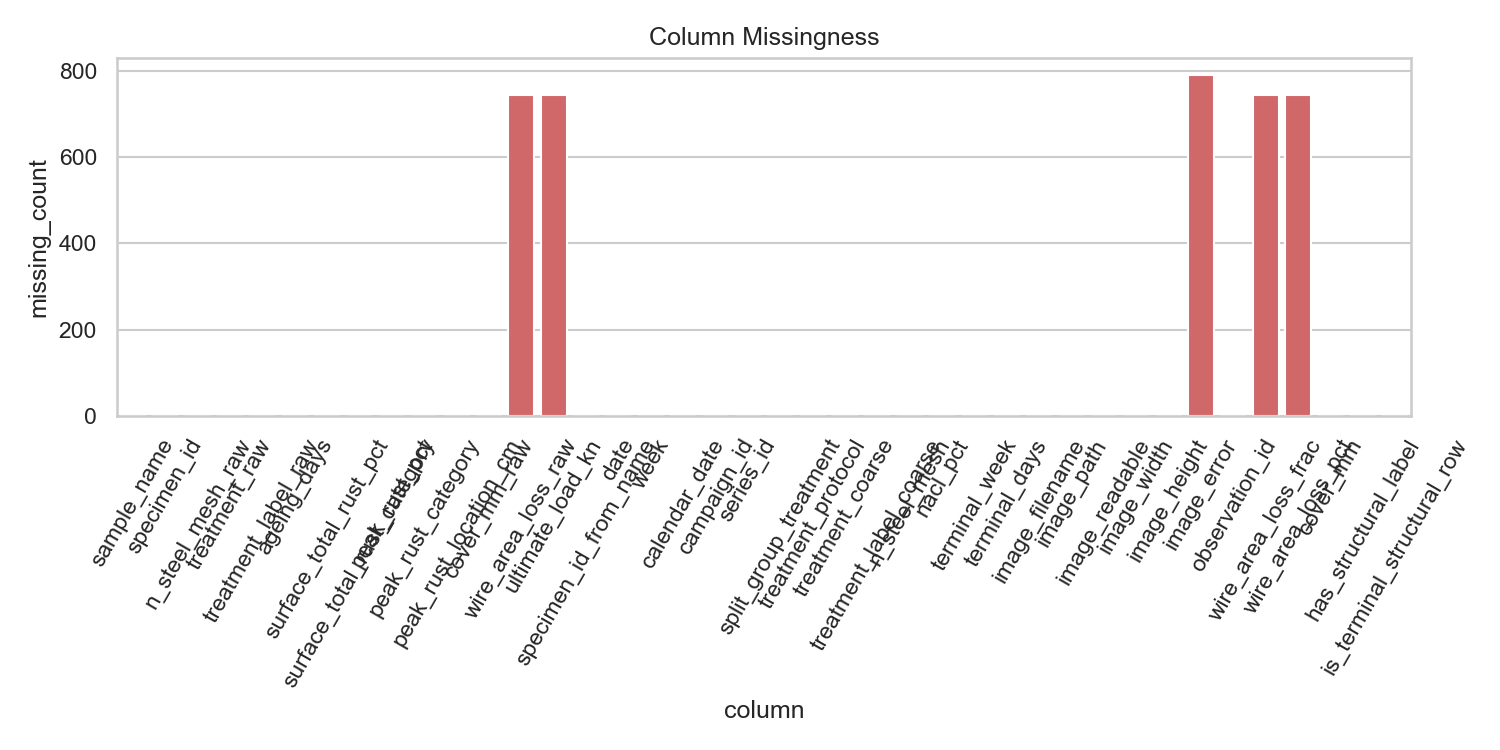
\includegraphics[width=0.88\textwidth]{outputs/eda/figures/missingness.png}\\[0.9em]
    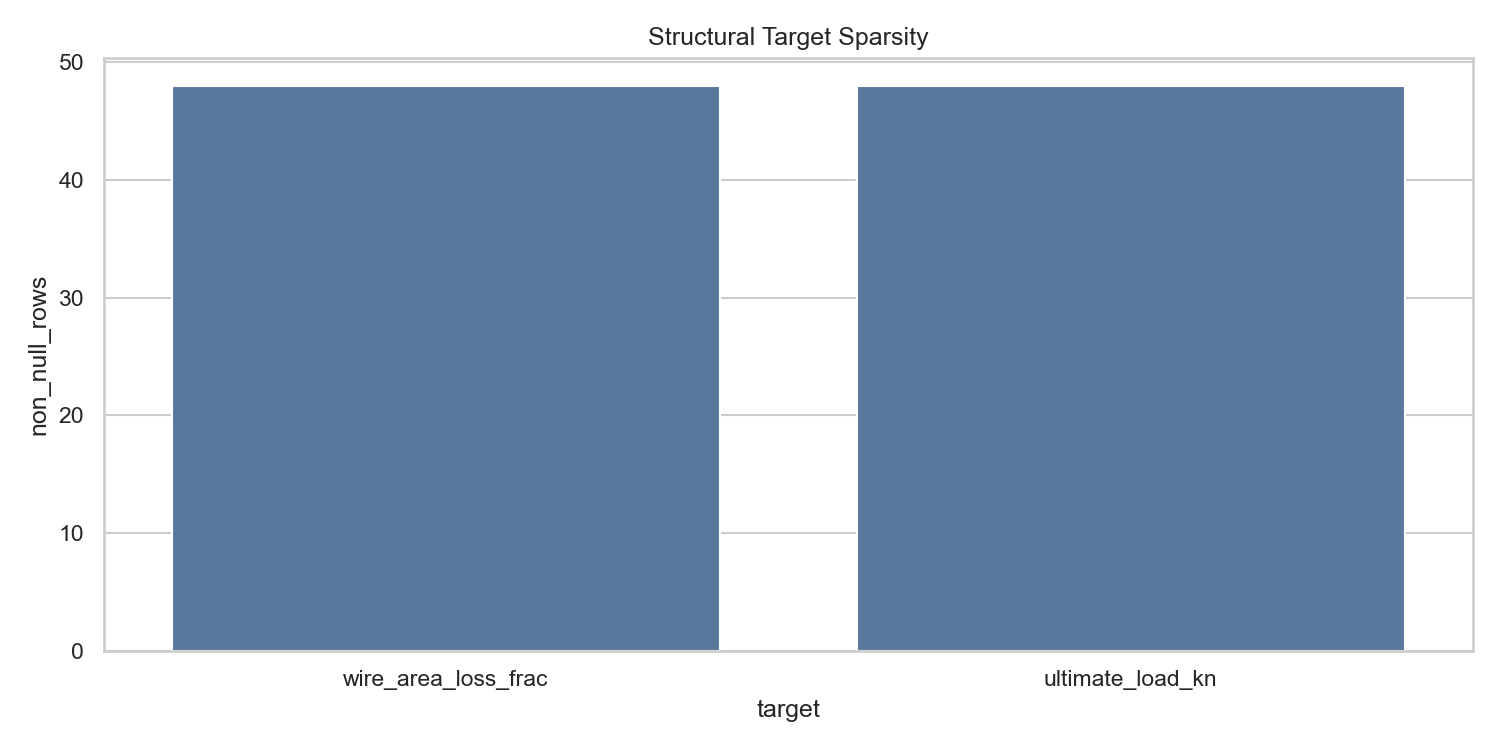
\includegraphics[width=0.70\textwidth]{outputs/eda/figures/structural_target_sparsity.png}
    \caption{Dataset availability and supervision constraints. Top: column-wise missing counts in the aligned master table. Bottom: non-null counts for the two structural targets, \texttt{wire\_area\_loss\_frac} and \texttt{ultimate\_load\_kn}.}
    \label{figsec:data-availability}
\end{figure}

The top panel is a data-availability result, not a corrosion result: it shows that the visible-corrosion variables are dense while the structural quantities are sparse. The bottom panel narrows that observation to the terminal structural labels. In the aligned tables, the structural subset comprises 48 labelled rows, effectively one terminal observation per specimen. The justified conclusion is that direct supervised end-to-end RUL estimation is not supported by the repository as it stands. These plots do not justify any claim about treatment efficacy, corrosion kinetics, or model quality by themselves; they justify the staged problem formulation.

\subsection{Microscopy and material-inspection figures}

No verified microscopy figures were found under \path{Data/}, \path{outputs/}, or \path{Documentation/}. No cross-sectional images, polished-sample micrographs, SEM images, or annotated pit-depth maps are present in the repository. Hidden damage is therefore observed only indirectly through terminal structural labels and model-derived proxies. That absence should stay explicit in any meeting discussion because it limits how strongly internal damage mechanisms can be interpreted from visible surface imagery alone.

\subsection{Corrosion progression over time}

The temporal figures are the strongest direct evidence that visible corrosion evolves over the observation window, but they also show that progression is heterogeneous and not strictly monotone for every specimen.

\begin{figure}[t]
    \centering
    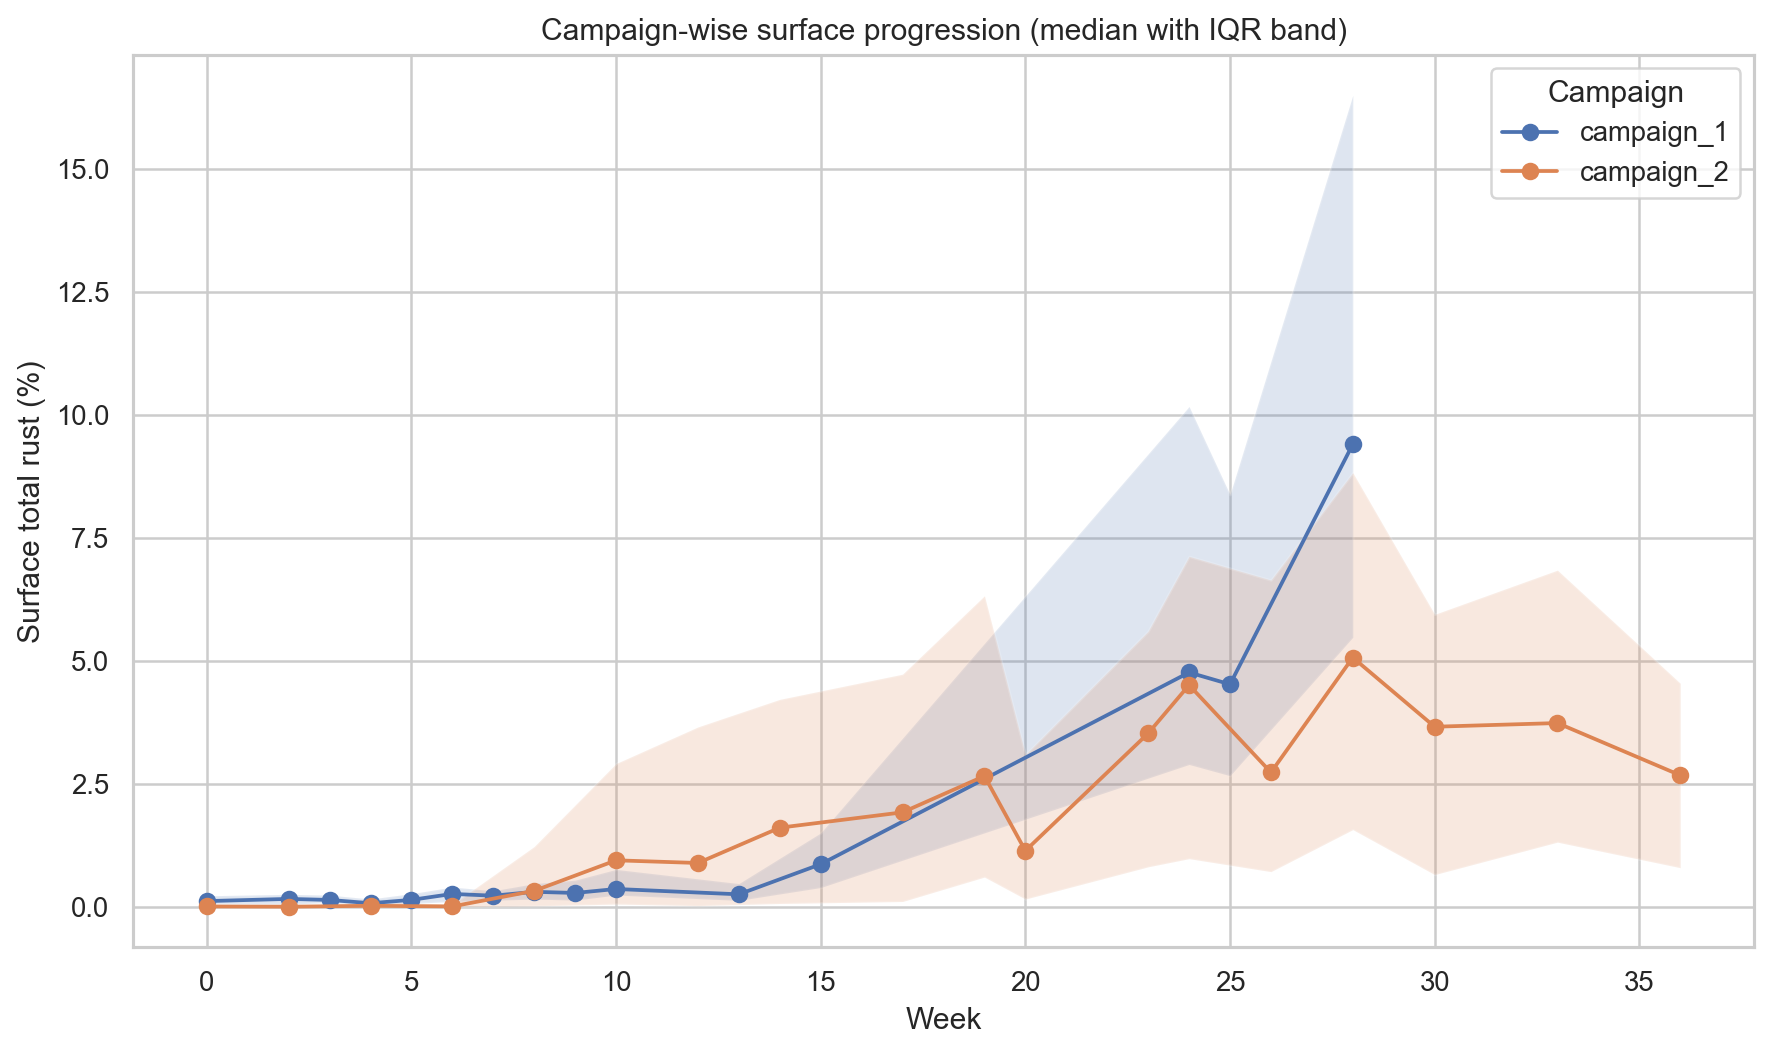
\includegraphics[width=0.90\textwidth]{outputs/diagnostics/figures/temporal/campaign_surface_progression_median_iqr.png}
    \caption{Campaign-level surface-rust progression. The x-axis is exposure week and the y-axis is \texttt{surface\_total\_rust\_pct}; each campaign is summarized by its median trajectory with an interquartile band.}
    \label{figsec:campaign-progress}
\end{figure}

Figure~\ref{figsec:campaign-progress} compresses many specimen trajectories into a readable campaign summary. Both campaigns show upward central tendency, but the campaigns are not directly comparable as a pure treatment experiment: \path{configs/specimen_mapping.yaml} assigns different terminal durations, mesh counts, and NaCl settings to campaign~1 and campaign~2, and campaign~2 also extends to week~36 while campaign~1 ends at week~28. The figure therefore supports the existence of visible-corrosion growth and campaign-level differences in spread, but it does not isolate a causal treatment effect.

\begin{figure}[t]
    \centering
    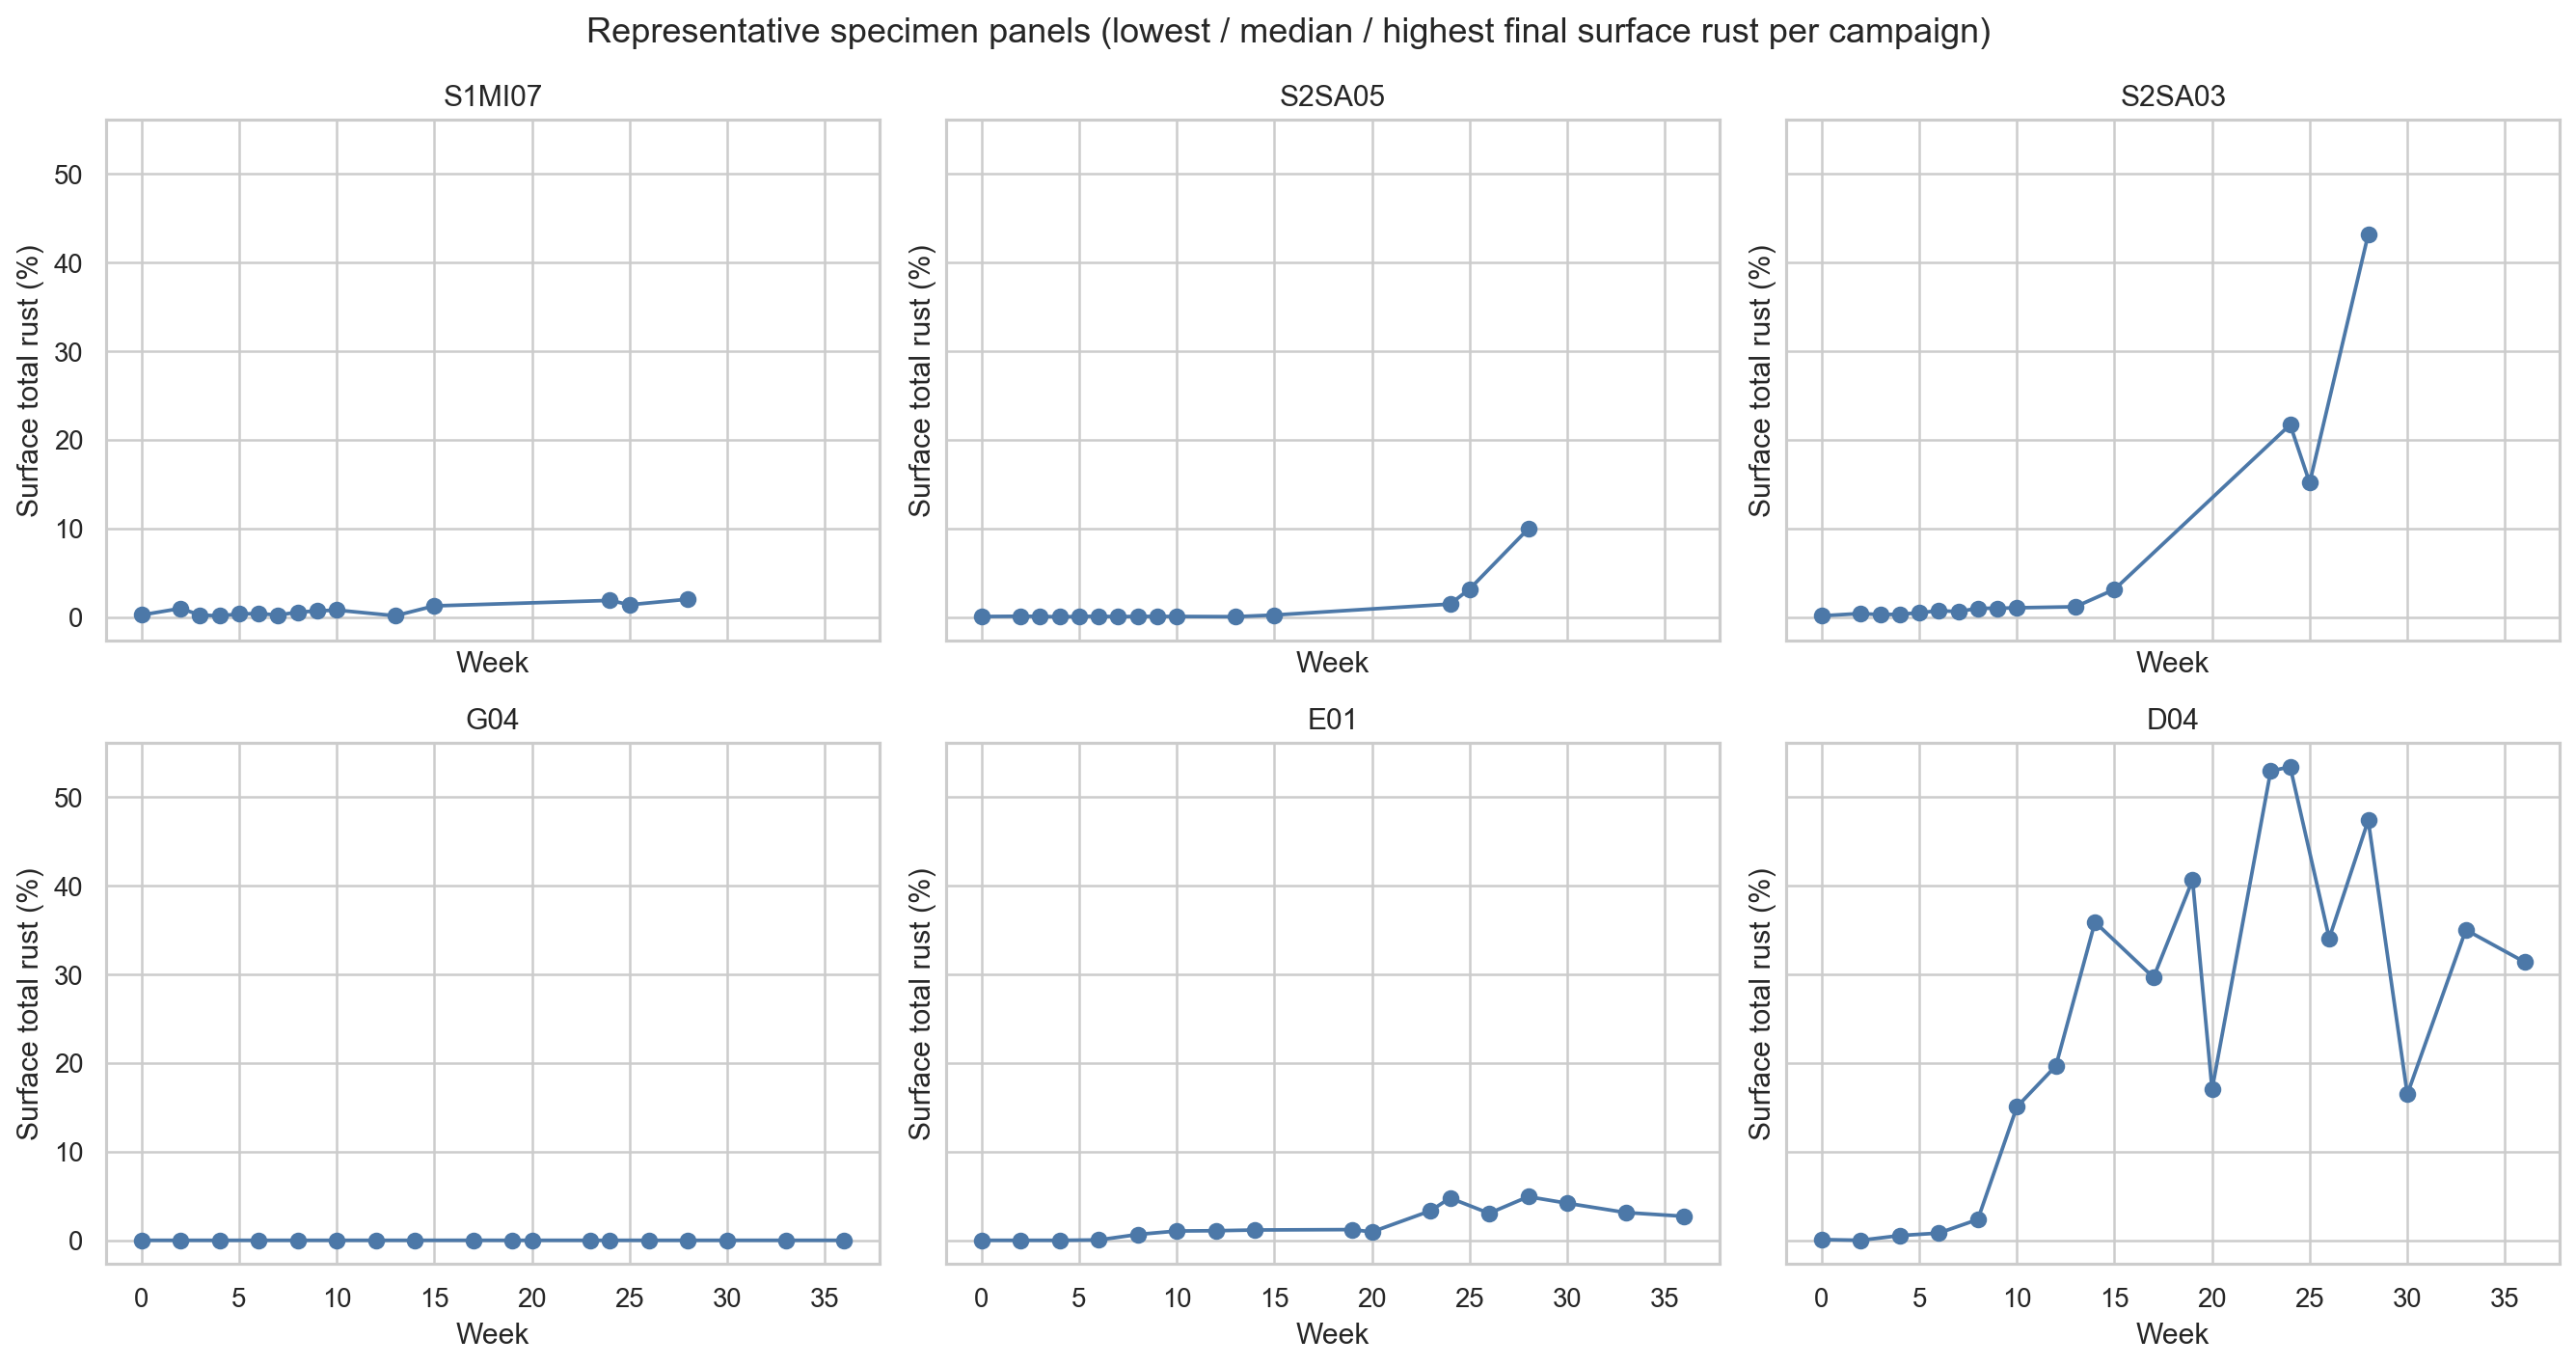
\includegraphics[width=0.92\textwidth]{outputs/diagnostics/figures/temporal/representative_specimen_surface_panels.png}
    \caption{Representative specimen-level surface trajectories selected by the diagnostics script as lowest, median, and highest final \texttt{surface\_total\_rust\_pct} within each campaign.}
    \label{figsec:representative-panels}
\end{figure}

This figure shows what the campaign medians hide. \texttt{G04} stays essentially at zero throughout 36 weeks, \texttt{S1MI07} and \texttt{E01} remain low to moderate, and \texttt{S2SA03} and \texttt{D04} exhibit late acceleration with short-term reversals. The reader can infer specimen heterogeneity and either measurement or segmentation variability. The reader should not over-claim a smooth physical corrosion law from these panels, because several curves plateau or decline between adjacent weeks.

\begin{figure}[t]
    \centering
    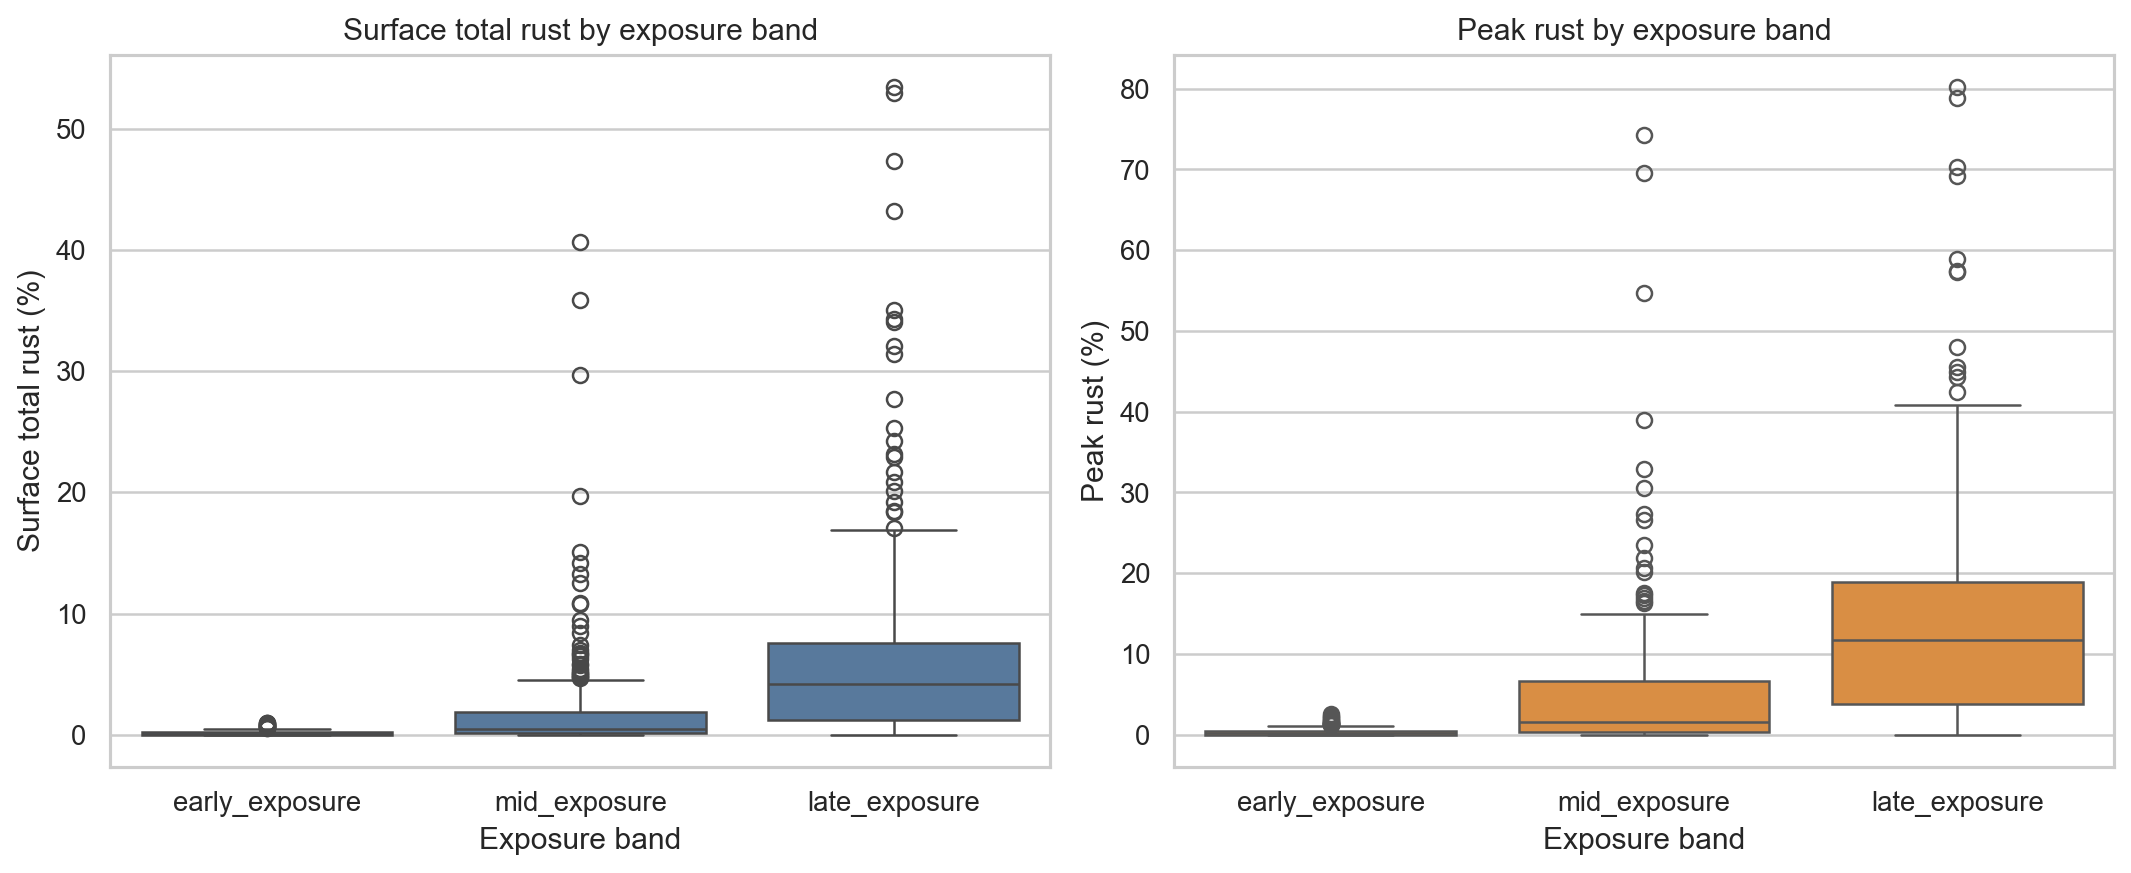
\includegraphics[width=0.92\textwidth]{outputs/diagnostics/figures/temporal/exposure_band_target_boxplots.png}
    \caption{Visible-corrosion distributions grouped into early-, mid-, and late-exposure bands. The left panel shows \texttt{surface\_total\_rust\_pct}; the right panel shows \texttt{peak\_rust\_pct}.}
    \label{figsec:exposure-bands}
\end{figure}

The exposure-band view confirms the same progression at a coarser aggregation level. In \path{outputs/diagnostics/tables/exposure_band_summary.csv}, the median \texttt{surface\_total\_rust\_pct} rises from 0.073 in early exposure to 0.478 in mid exposure and 4.184 in late exposure. The corresponding \texttt{peak\_rust\_pct} medians increase from 0.218 to 11.681. The widening spread in the late band matters because it warns against reducing corrosion progression to a single mean curve or assuming that later exposure implies the same severity for every specimen.

\subsection{Image-processing pipeline and spatial strip features}

The repository does not save intermediate segmentation masks or strip overlays as figures. The recoverable figure evidence for the image-processing stage is therefore downstream: feature-target associations and feature-feature redundancy.

\begin{figure}[t]
    \centering
    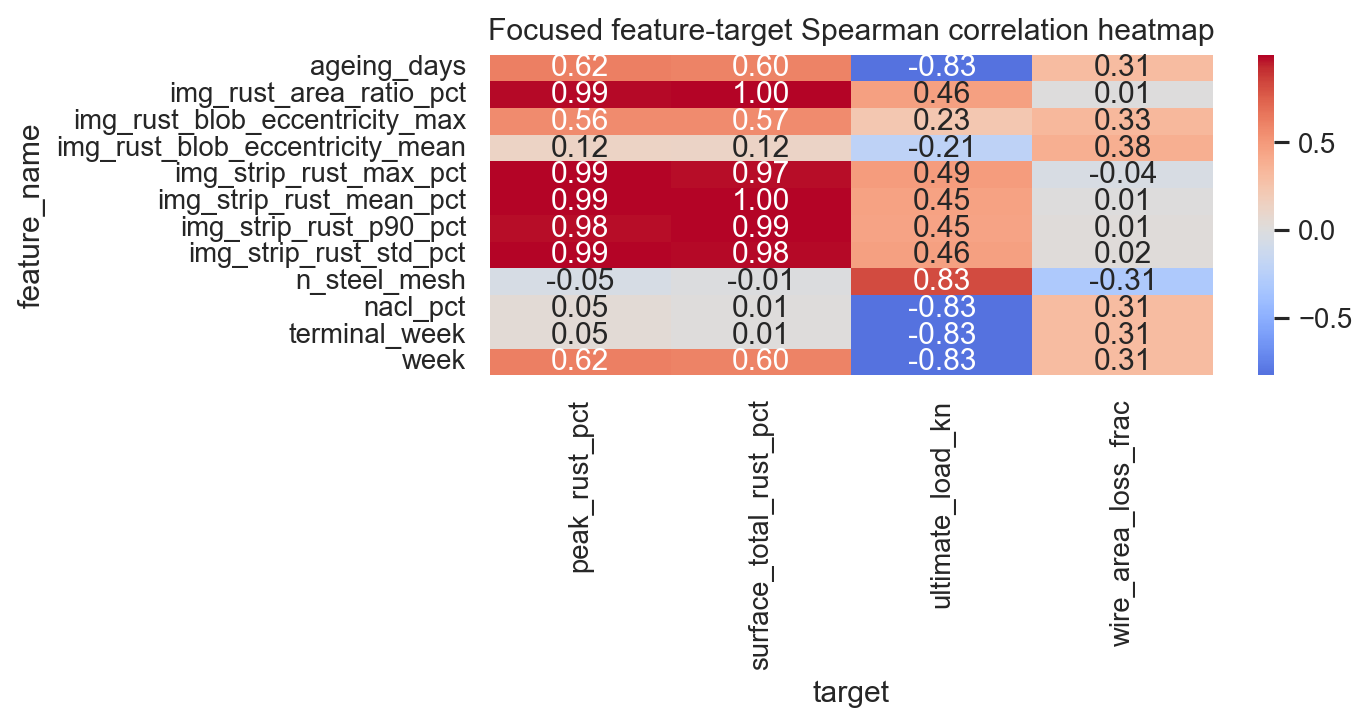
\includegraphics[width=0.88\textwidth]{outputs/diagnostics/figures/features/feature_target_correlation_heatmap.png}
    \caption{Focused Spearman correlations between selected engineered features and the four main targets.}
    \label{figsec:feature-target}
\end{figure}

This heatmap is the most direct summary of what the extracted image features encode. The visible-corrosion targets are almost tautologically captured by rust-area and strip-rust features: \texttt{img\_rust\_area\_ratio\_pct} has Spearman 0.9996 with \texttt{surface\_total\_rust\_pct}, while strip features such as \texttt{img\_strip\_rust\_std\_pct}, \texttt{img\_strip\_rust\_max\_pct}, and \texttt{img\_strip\_rust\_mean\_pct} are all above 0.98 for \texttt{peak\_rust\_pct}. The structural targets are much weaker. The strongest listed correlation with \texttt{wire\_area\_loss\_frac} is \texttt{img\_rust\_blob\_eccentricity\_mean} at about 0.38, and the strongest association with \texttt{ultimate\_load\_kn} in the selected table is the negative correlation with time-linked experimental metadata. The figure strongly supports the visible-corrosion stage, but it does not establish that the image pipeline alone predicts internal damage.

\begin{figure}[t]
    \centering
    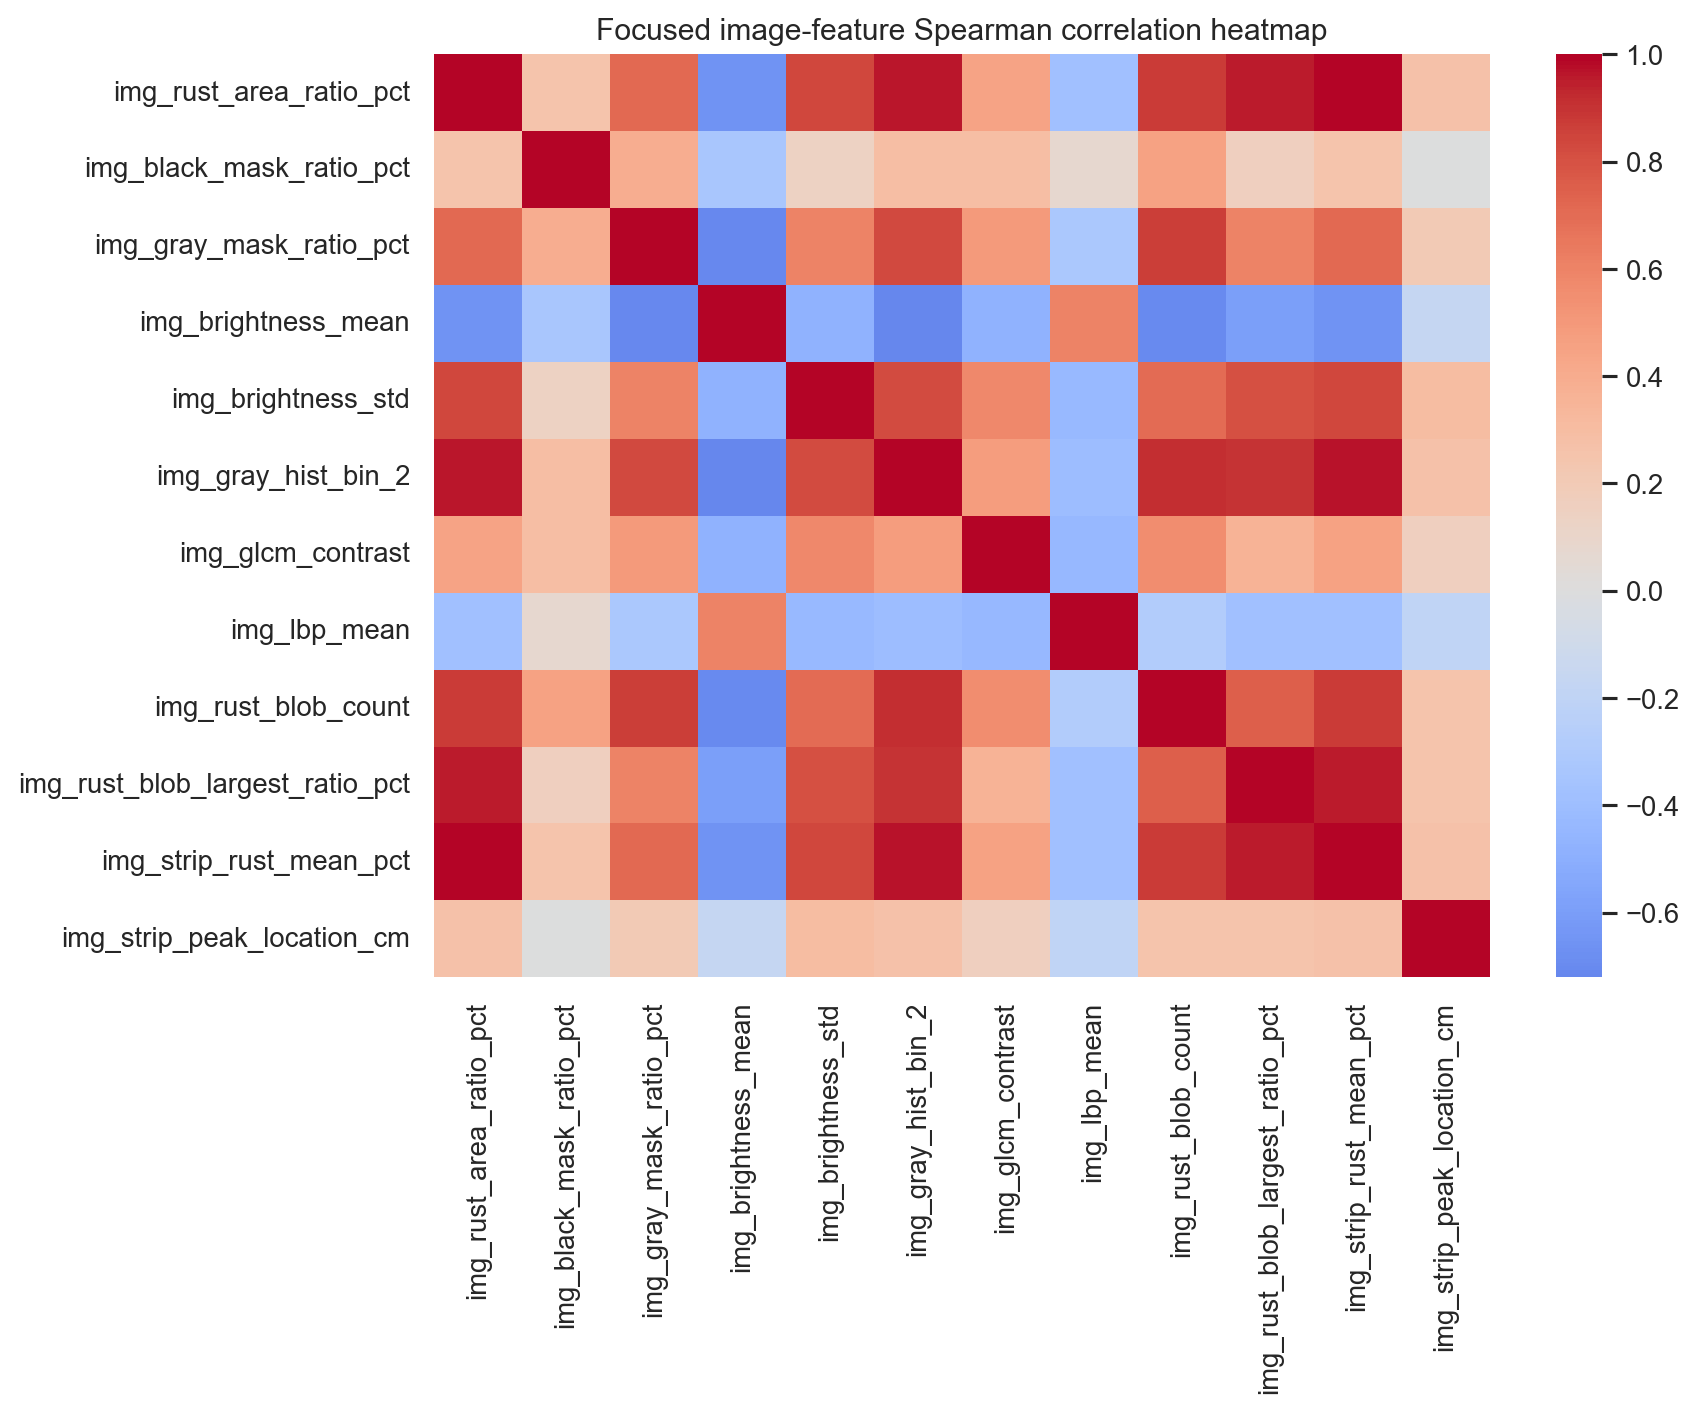
\includegraphics[width=0.82\textwidth]{outputs/diagnostics/figures/features/image_feature_correlation_heatmap.png}\\[0.8em]
    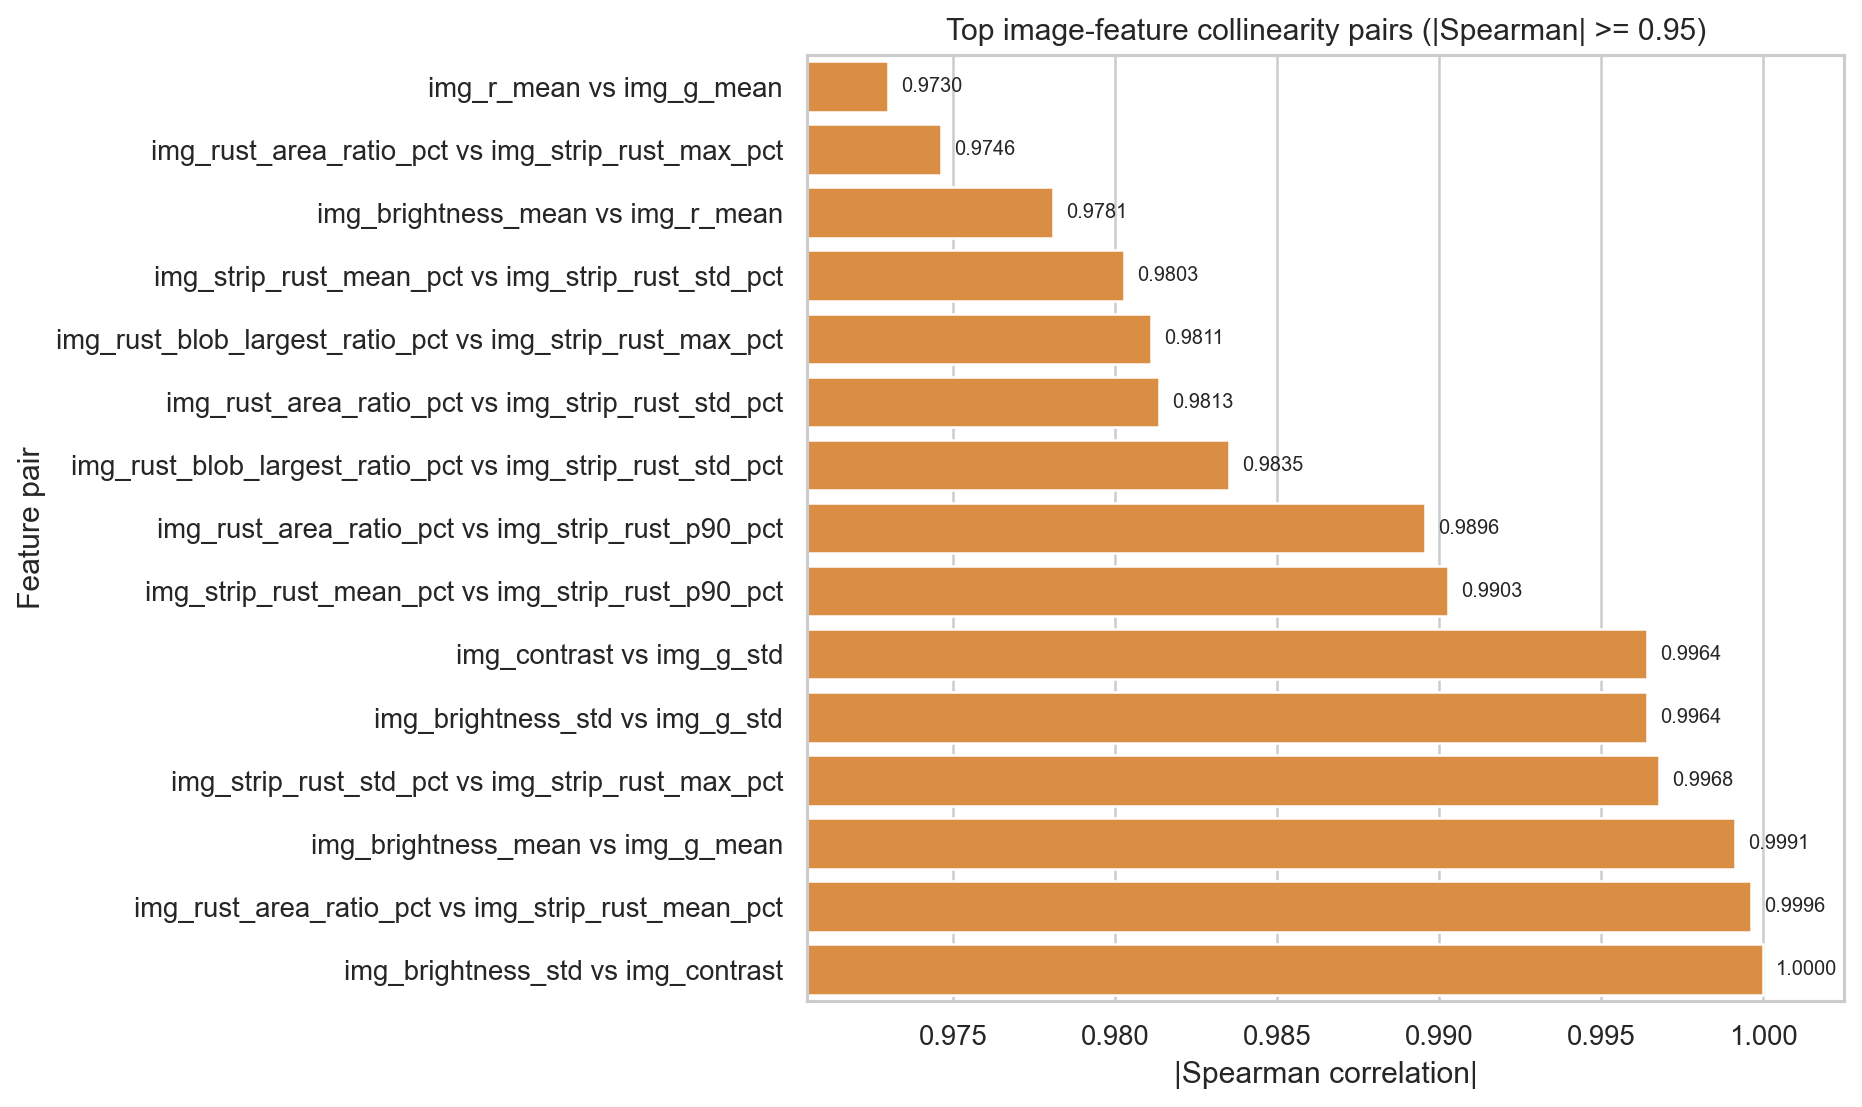
\includegraphics[width=0.88\textwidth]{outputs/diagnostics/figures/features/high_collinearity_pairs.png}
    \caption{Feature redundancy within the image-processing stage. Top: focused Spearman correlation heatmap for selected image features. Bottom: top feature pairs with absolute Spearman correlation at or above 0.95.}
    \label{figsec:image-redundancy}
\end{figure}

The top panel shows that mask ratios, grayscale statistics, rust-blob features, and strip summaries do not behave as independent signals. The bottom panel makes that explicit: the diagnostics tables contain 36 high-collinearity pairs, including exact or near-exact duplicates such as \texttt{ageing\_days} versus \texttt{week}, \texttt{img\_brightness\_std} versus \texttt{img\_contrast}, and \texttt{img\_rust\_area\_ratio\_pct} versus \texttt{img\_strip\_rust\_mean\_pct}. This is the available figure evidence for the spatial strip-based family: the repository exposes strip-derived summary variables such as mean, max, p90, standard deviation, and peak location, but it does not export a strip-by-strip corrosion map. Interpretation should therefore stay at the level of strip summary statistics rather than spatially resolved pit morphology.

\subsection{Mechanical-target diagnostics and cross-campaign robustness}

No direct mechanical-test photographs or load-frame figures are present in the repository. The mechanical-test family is represented indirectly through the terminal targets \texttt{ultimate\_load\_kn} and \texttt{wire\_area\_loss\_frac}, together with benchmark diagnostics.

\begin{figure}[t]
    \centering
    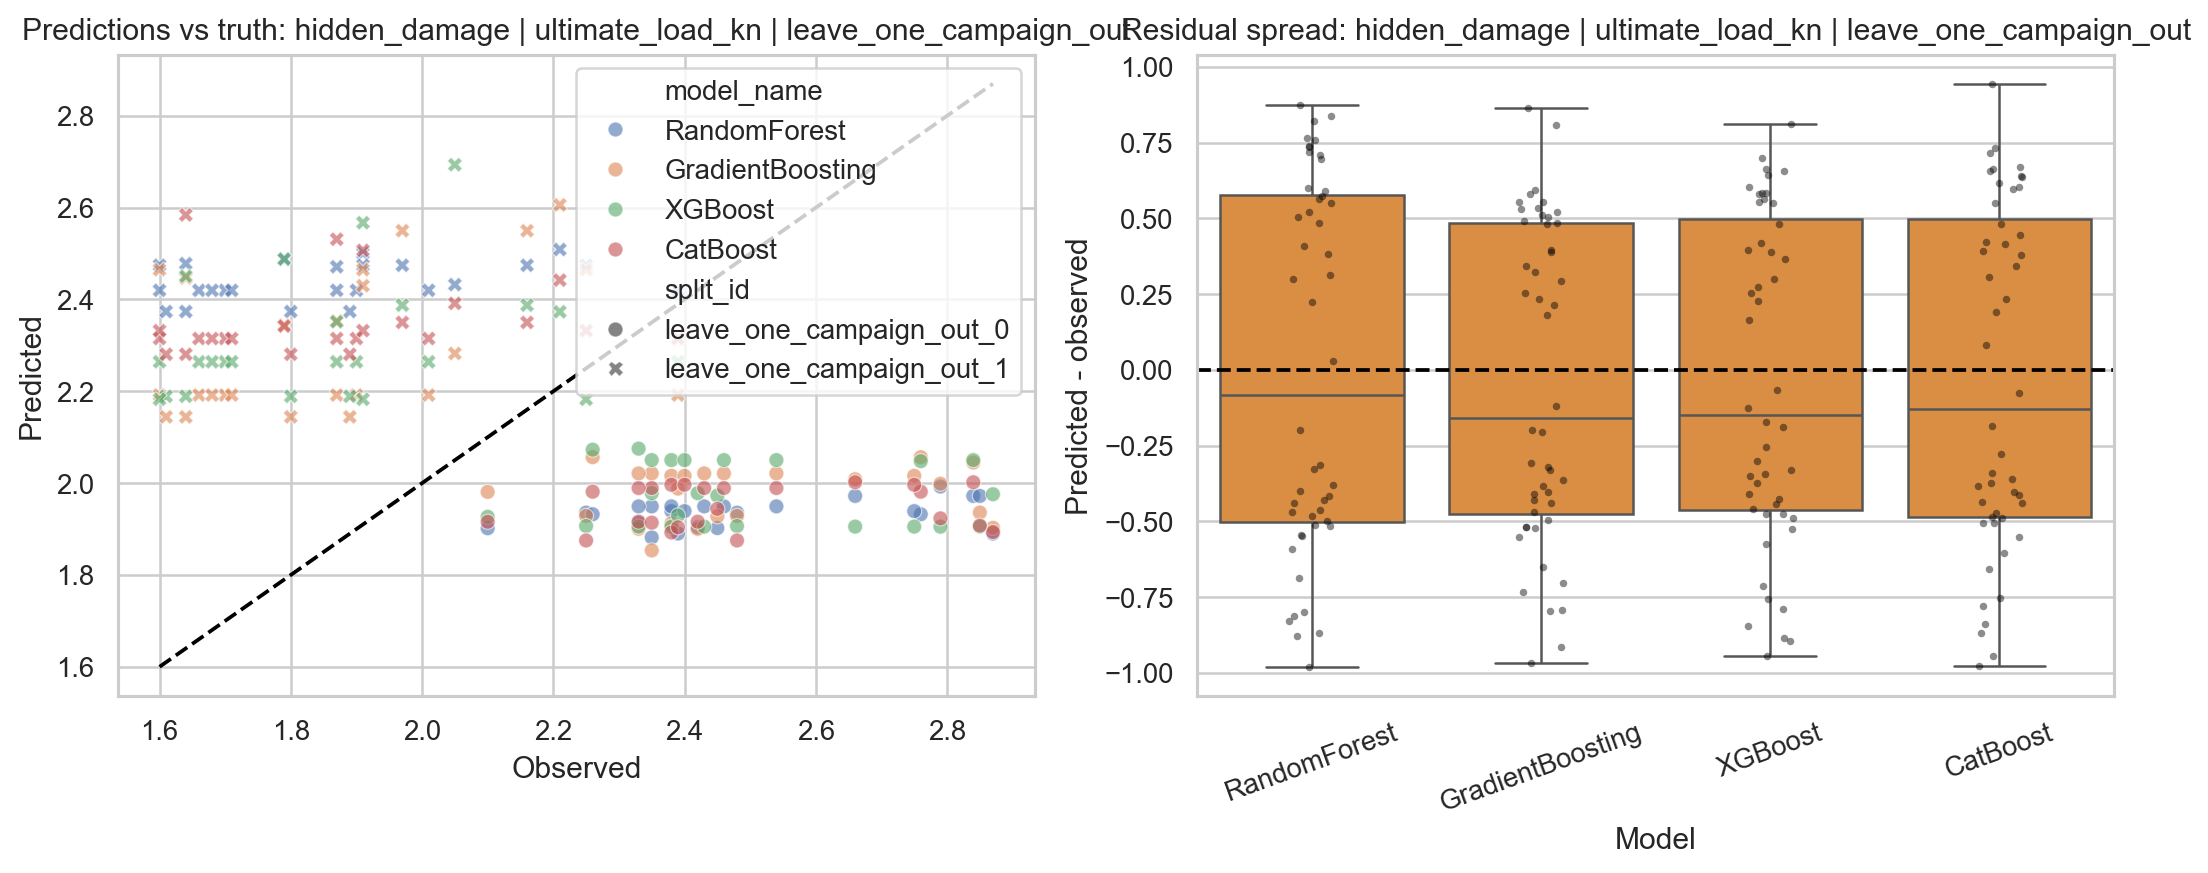
\includegraphics[width=0.94\textwidth]{outputs/diagnostics/figures/benchmarks/predictions/hidden_damage/ultimate_load_kn/ultimate_load_kn_leave_one_campaign_out_prediction_diagnostics.png}
    \caption{Leave-one-campaign-out prediction diagnostics for the hidden-damage target \texttt{ultimate\_load\_kn}. The left panel plots observed versus predicted values for four benchmark models; the right panel shows residual distributions by model.}
    \label{figsec:ultimate-loco}
\end{figure}

This is the closest available figure to a mechanical-test result figure. The diagonal in the left panel marks perfect agreement. All four models compress predictions into relatively narrow bands, and the residual boxplots remain wide. That pattern matches the benchmark tables: grouped performance is substantially better than leave-one-campaign-out performance for \texttt{ultimate\_load\_kn}. The figure therefore shows that campaign-shift generalization is unresolved. It does not show laboratory failure modes or validate a mechanistic link between surface corrosion and ultimate load.

\begin{figure}[t]
    \centering
    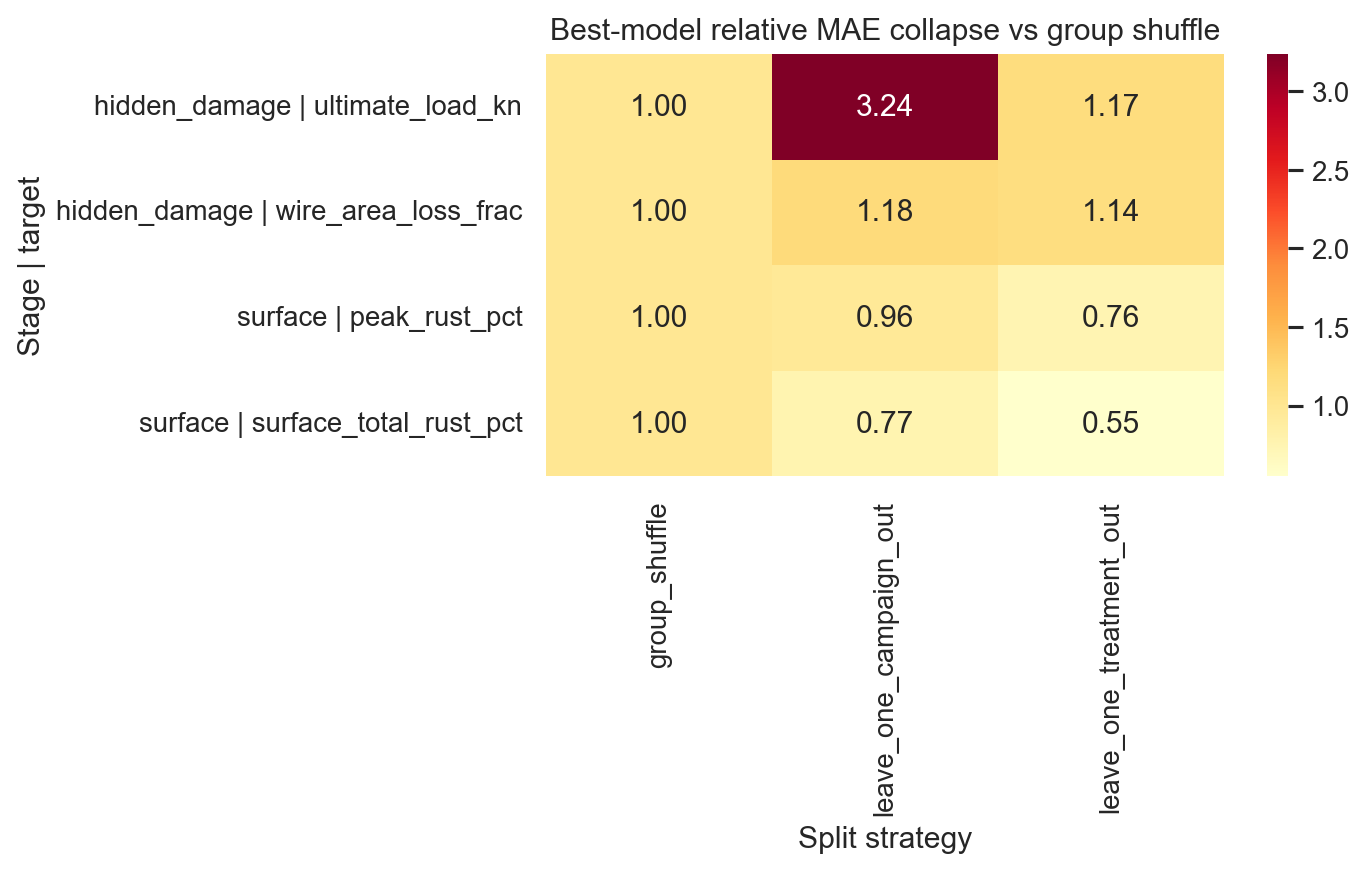
\includegraphics[width=0.88\textwidth]{outputs/diagnostics/figures/benchmarks/best_model_relative_mae_collapse_heatmap.png}
    \caption{Relative MAE inflation when the split strategy becomes harder. Values above 1 indicate worse performance than the grouped baseline for the corresponding best model.}
    \label{figsec:collapse-heatmap}
\end{figure}

The relative-MAE heatmap is the clearest cross-stage robustness summary in the repository. Surface targets remain comparatively stable across the tested split strategies, whereas \texttt{ultimate\_load\_kn} rises to about 3.24 times its grouped MAE under leave-one-campaign-out evaluation. \texttt{wire\_area\_loss\_frac} degrades less in absolute MAE but remains weak in rank-order behaviour. The figure matters because it separates easy within-dataset success from robust transfer performance.

\begin{figure}[t]
    \centering
    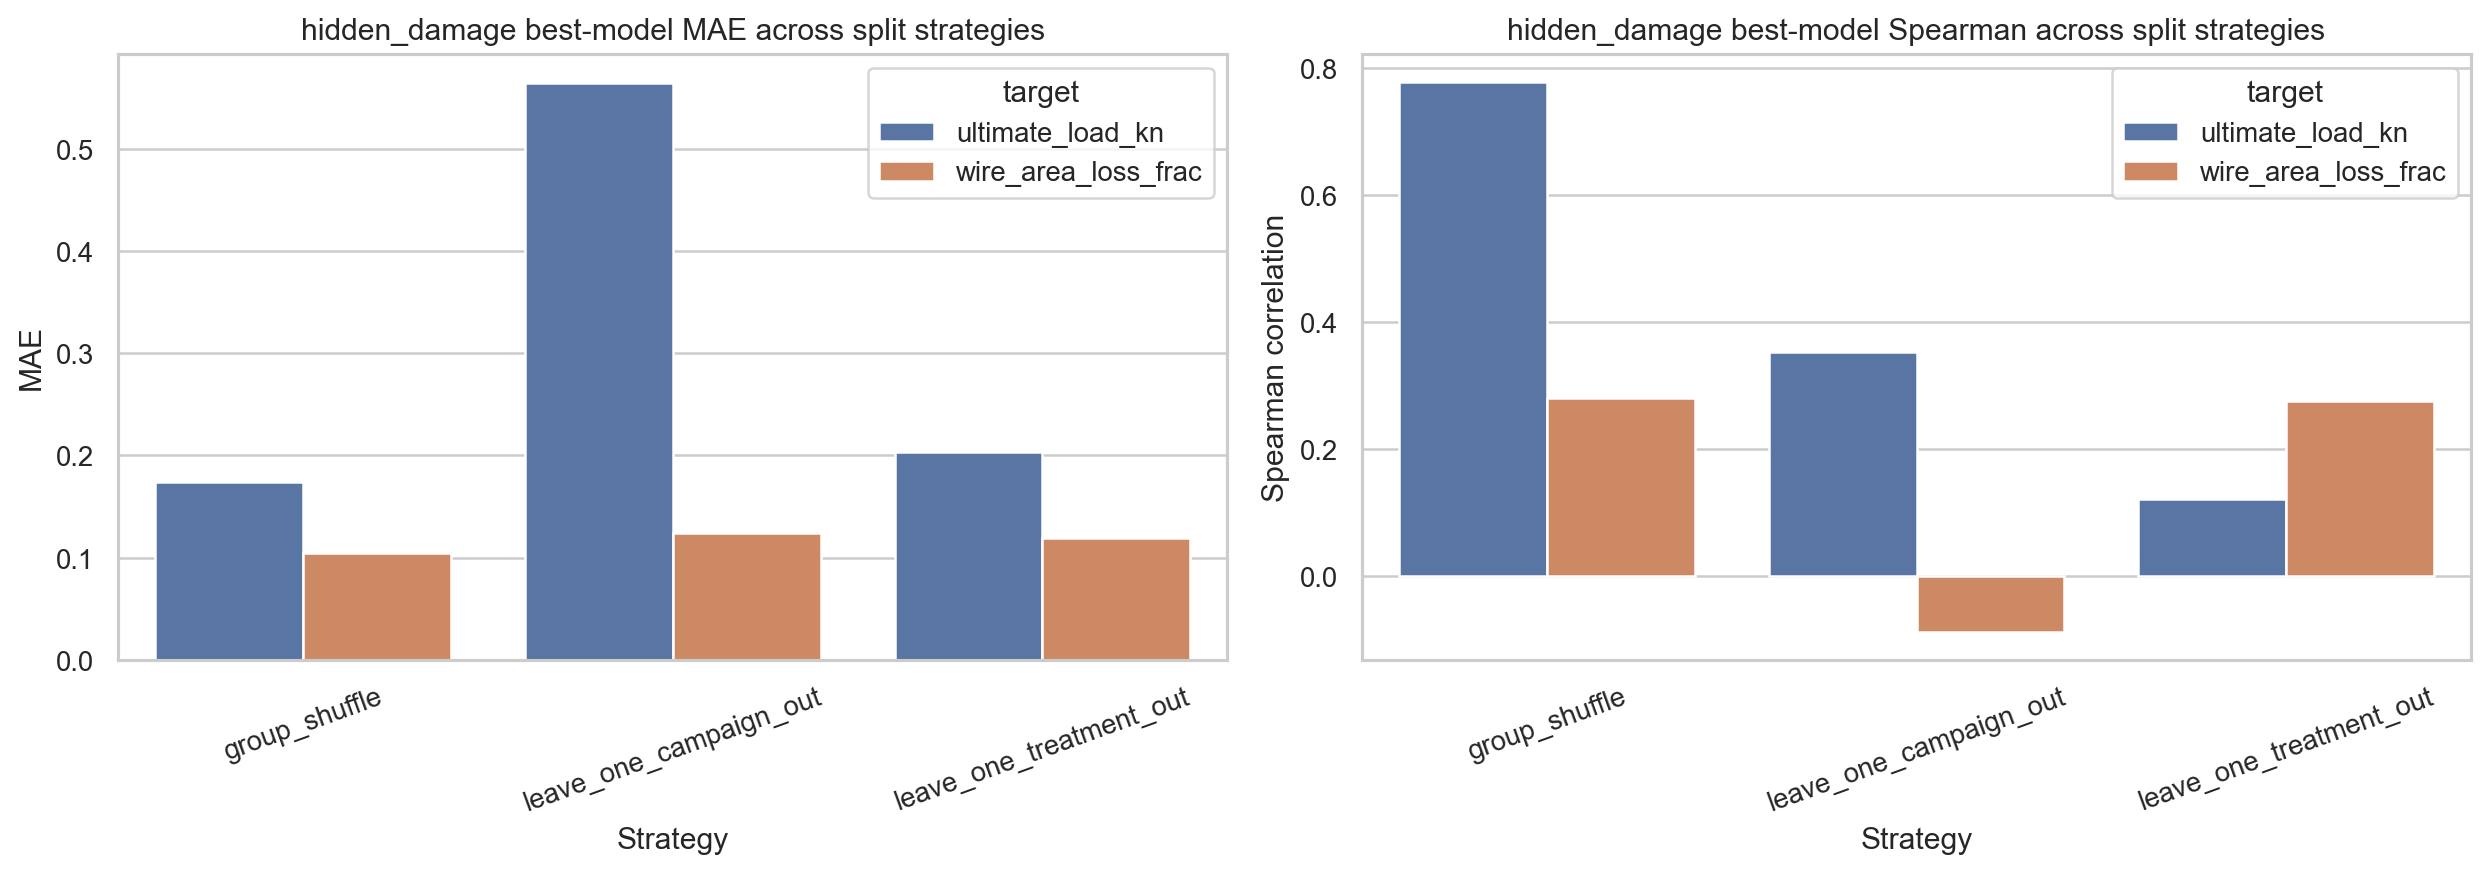
\includegraphics[width=0.88\textwidth]{outputs/diagnostics/figures/benchmarks/hidden_damage_best_model_strategy_robustness.png}
    \caption{MAE and Spearman robustness of the selected hidden-damage models across grouped, leave-one-treatment-out, and leave-one-campaign-out evaluation.}
    \label{figsec:hidden-robustness}
\end{figure}

This figure resolves the structural weakness at the selected-model level. According to \path{outputs/models/hidden_damage/best_models.csv} and the selected-feature files, the final models for both structural targets use the \texttt{metadata\_only} feature set with eight metadata variables. That is a defensible model-selection outcome, but it is also a limitation: the current structural stage is leveraging campaign, treatment, and timing descriptors more clearly than image-derived hidden-damage signatures. The figure supports a cautious claim of benchmarking progress; it does not support a strong claim of image-based hidden-damage prediction.

\subsection{Degradation modelling and proxy-RUL status}

\begin{figure}[t]
    \centering
    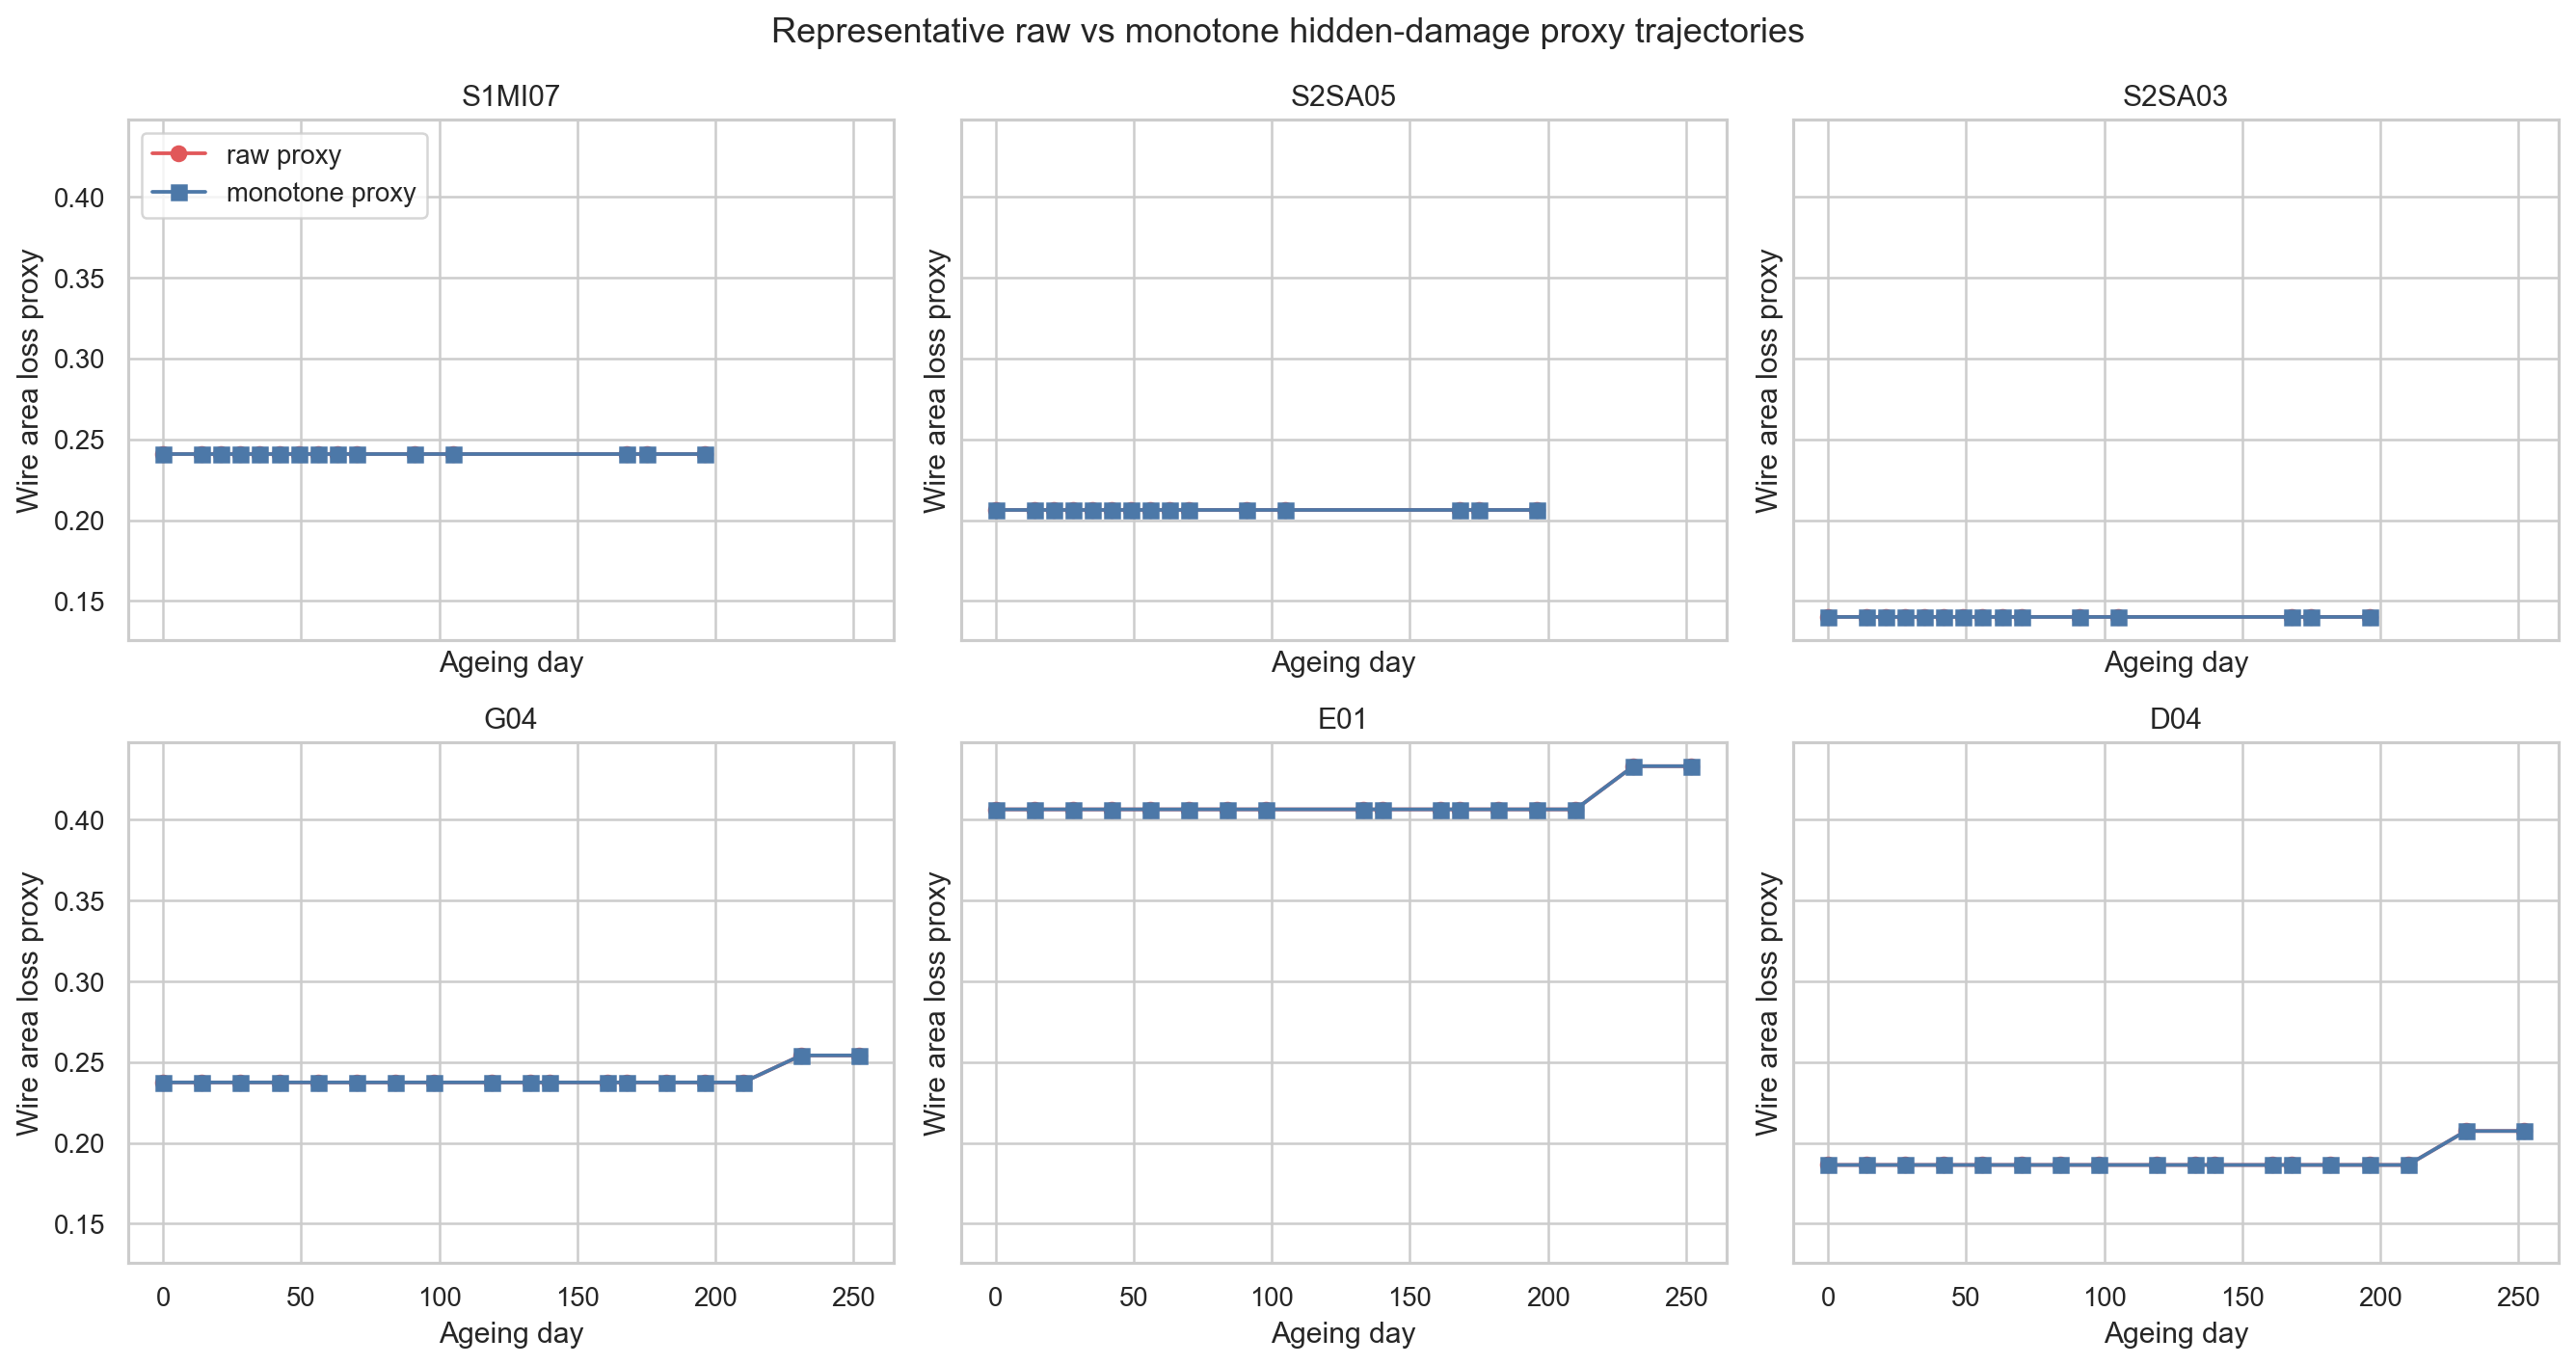
\includegraphics[width=0.92\textwidth]{outputs/diagnostics/figures/degradation/degradation_raw_vs_monotone_representative.png}
    \caption{Representative raw and monotone-smoothed hidden-damage proxy trajectories. The x-axis is ageing day and the y-axis is the wire-area-loss proxy produced before threshold analysis.}
    \label{figsec:degradation-monotone}
\end{figure}

This figure explains why monotone projection was introduced before proxy-RUL thresholding. Several panels are nearly flat for long intervals and change only near late observations; the monotone proxy removes local reversals and enforces non-decreasing behaviour. That is a modelling convenience consistent with a degradation interpretation, but it is not proof of a physical law. The repository fit summaries show that multiple curve families fit the smoothed trajectories very closely, so this figure should be read as stabilization rather than mechanistic validation.

\begin{figure}[t]
    \centering
    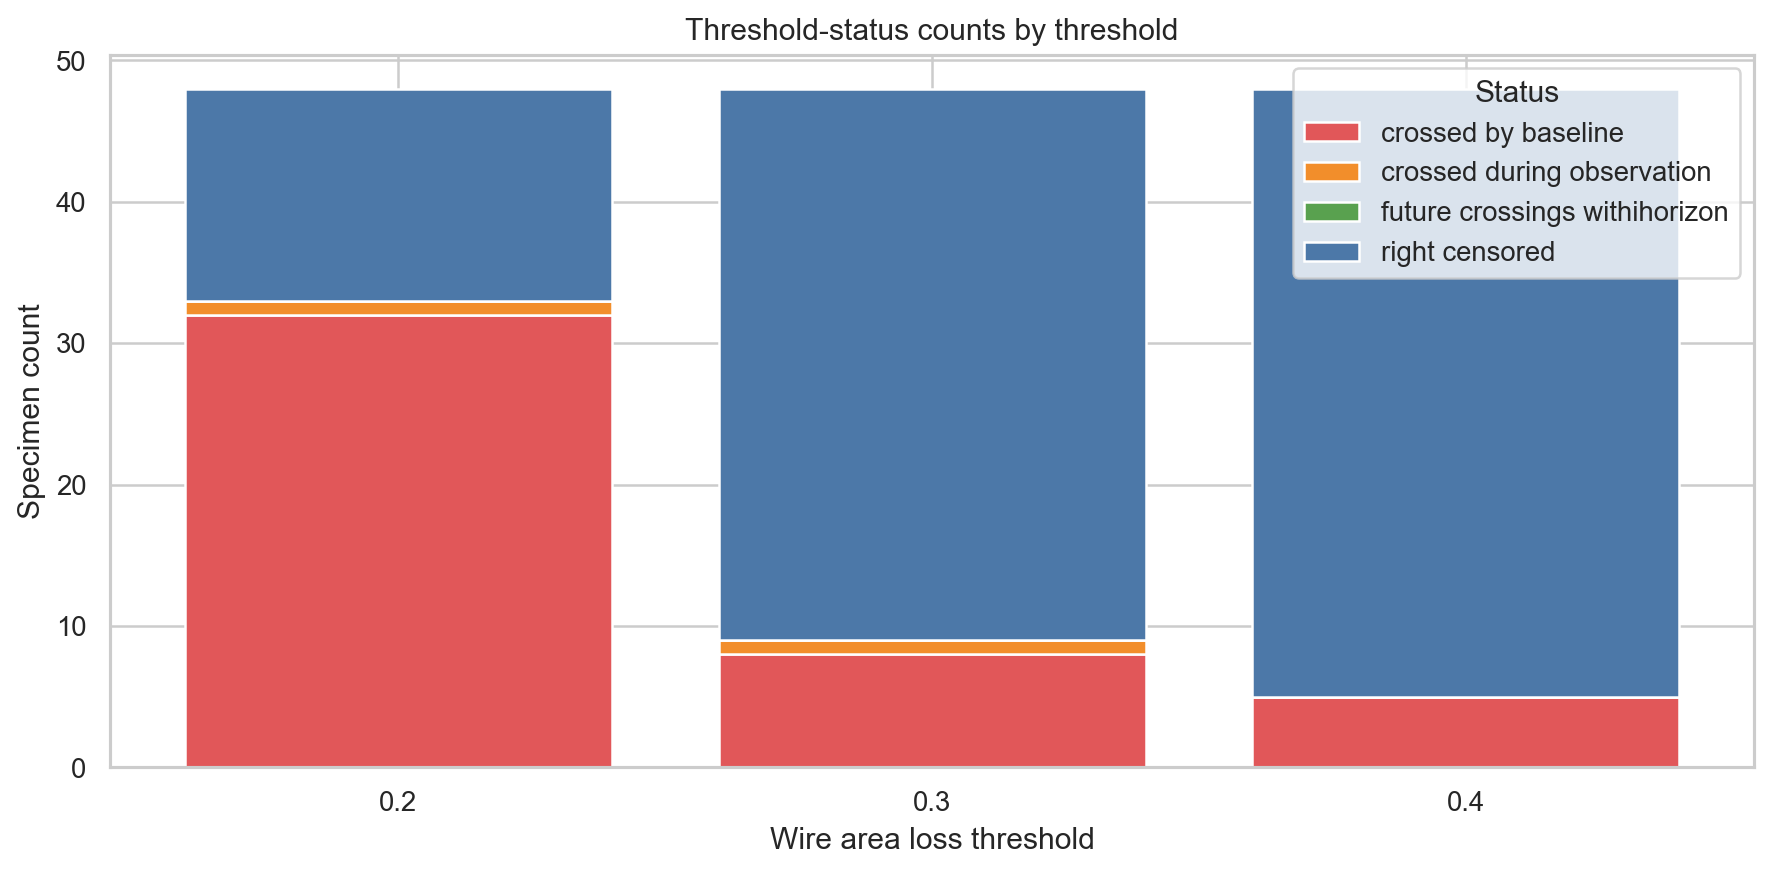
\includegraphics[width=0.88\textwidth]{outputs/diagnostics/figures/proxy/proxy_threshold_status_counts.png}
    \caption{Threshold-status counts for the proxy-RUL stage across wire-area-loss thresholds 0.20, 0.30, and 0.40.}
    \label{figsec:proxy-status}
\end{figure}

This is the clearest current summary of the proxy stage. At threshold 0.20, 32 of 48 specimens are already above threshold at baseline and one more crosses during observation; at 0.30 the counts are 8 and 1; at 0.40 they are 5 and 0. The future-crossing-within-horizon category is zero at all three thresholds. The justified conclusion is that the current proxy layer is mostly a threshold-status accounting exercise with heavy right censoring. It should not be presented as an operational residual-life estimator.

\subsection{Figure Audit Notes}

\begin{itemize}
    \item \textbf{Included figures.} This section uses 15 verified image files: 2 raw specimen images under \path{Data/Images_dataset/} and 13 generated plots under \path{outputs/eda/figures/} and \path{outputs/diagnostics/figures/}. The included generated families cover data availability, temporal corrosion progression, feature-target relations, feature redundancy, structural benchmark diagnostics, degradation smoothing, and proxy-threshold status.
    \item \textbf{Unused but verified figures.} 81 generated report figures remain unused in this section. They are mostly appendix-level companions: additional distribution diagnostics, treatment-group plots, model-comparison plots, ranked feature-importance plots, and legacy stage outputs under \path{outputs/models/} and \path{outputs/improvements/baseline_snapshot/}. The remaining 790 raw specimen files were not promoted here; 789 are readable source observations and one is the unreadable orphan flagged by the audit.
    \item \textbf{Missing or broken references.} Every \texttt{includegraphics} path in this file was verified on disk before writing. No included reference is broken. One raw file, \path{Data/Images_dataset/E01-20240508-17W.png}, is flagged as unreadable in \path{outputs/audit/issues_log.csv} and was therefore not promoted.
    \item \textbf{Ambiguous figure families.} Treatment-group figures such as \path{outputs/diagnostics/figures/temporal/treatment_surface_progression_median.png} and \path{outputs/diagnostics/figures/degradation/degradation_grouped_by_treatment.png} are interpretable only with an explicit warning that treatment labels are entangled with campaign design in \path{configs/specimen_mapping.yaml}. Legacy outputs such as \path{outputs/models/degradation/degradation_subset_trajectories.png} and \path{outputs/models/proxy_rul/proxy_rul_right_censored.png} remain real but under-specified relative to the newer diagnostics figures.
    \item \textbf{Figures needing regeneration or stronger captions.} The repository currently lacks exported segmentation masks, strip overlays, microscopy images, and direct mechanical-test photographs. If those views are needed for the final report, they must be generated or added explicitly; they cannot be reconstructed defensibly from the current tree. Prediction-diagnostic and feature-importance figures promoted later should name the split strategy, target scale, and specimen-selection logic directly in the caption.
\end{itemize}

\end{document}
